\section{Theorie}

Die Ultraschalltechnik ist heutzutage ein wichtiges Element im Alltag.
Vor allem in der Medizin spielt die Ultraschalltechnick eine grundlegende Methode in der Therapie
und auch in der Diagnostik. In dem folgenden Versuch sollen grundlegende
Eigenschaften und Definitionen der Ultraschallechographie kennengelernt und
angewandt werden.

\subsection{Theoretische Grundlagen}

Der Ultraschall besitzt eine für den Menschen nicht wahrnehmbare Frequenzbereich
zwischen $\SI{20}{kHz}$ und $\SI{1}{GHz}$. Im Allgemeinen ist Schall eine
longitudinale Welle, die mittels Druckschwankungen weitergeleitet wird und durch
folgende Formel beschrieben werden kann:

\begin{equation}
  p(x,t) = p\ua{0} + v\ua{0}Z\cos{\omega t - kx} .
  \label{eqn:Druckwelle}
\end{equation}

Bei dem Faktor $Z$ handelt es sich um die akustische Impedanz, welche mithilfe der
Dichte und der Schallgeschwindigkeit des vorliegenden Stoffes beschrieben wird:

\begin{equation}
  Z = c \cdot \rho .
  \label{eqn:Impedanz}
\end{equation}

Schallwellen zeigen im Allgemeinen das selbe Verhalten wie elektromagnetische Wellen auf,
jedoch ist bei Schwalwellen aufgrund der Änderung von Druck und Dichte die
Phasengeschwindigkeit materialabhängig.

Bei Schallwellen muss aufgrund von unterschiedlichen Eigenschaften zwischen
gasförmigen oder flüssigen Medien und Festkörpern unterschieden werden. In Gasen und
Flüssigkeiten treten lediglich Longitudinalwellen auf, sodass sich für die
Schallgeschwindigkeit folgende Relation ergibt:

\begin{equation}
  c\ua{Fl} = \sqrt{ \frac{1}{\kappa \cdot \rho} }.
  \label{eqn:C_Fl}
\end{equation}

$\kappa$ beschreibt dabei die Kompressibilität des Mediums.

Im Gegnsatz zu Gasen und Flüssigkeiten treten bei Festkörpen zusätzlich zu den
Longitudinalwellen noch Transversalwellen auf, sodass die Schallgeschwindigkeit
in Festkörpern allgemein richtungsabhängig ist. Für die Schallgeschwindigkeit ergibt
sich mit dem Elastizitätmodul $E$ damit folgender Zusammenhang:

\begin{equation}
  c\ua{Fe} = \sqrt{ \frac{E}{\rho}}.
  \label{eqn:C_Fk}
\end{equation}

Es muss beachtet werden, dass $c\ua{Fe}$ für Transversal- und
Longitudinalwellen unterschiedlich aussieht.

Bei der Betrachtung von Schallwellen in einem Medium ist zu Berücksichtigen, dass
im Allgemeinen immer ein Teil der Energie durch Absorption verloren geht. Deshalb
ist die Intensität der Welle als eine Funktion des Ortes und des
Absorptionskoeffizienten $\alpha$ beschreibbar:

\begin{equation}
  I(\su{x}) = I\ua{0} \cdot e^{-\alpha \su{x}} .
  \label{eqn:Intensität}
\end{equation}

Luft besitzt einen sehr großen Absorptionskoeffizienten, weshalb bei dem folgenden
Versuch immer ein Kontaktmittel verwendet wird. Bei dem Kontaktmittel handelt es sich
um bidestilliertes Wasser oder Hydrogel.

Während des Experimentes werden zwei verschiedenen Messmethoden verwendet, wovon
eine auf der reflektierten Welle und ein auf der transmittierten Welle basiert.
Der Reflexionskoeffizient $R$ beschreibt das Verhältnis der einfallenden und
reflektierten Intensität und ist von den akustischen Impedanzen der beiden
Medien ab, die die Grenzfläche bilden.

\begin{equation}
  R = \left( \frac{Z\ua{1} - Z\ua{2}}{Z\ua{1} + Z\ua{2}} \right)^2.
  \label{eqn:Reflexionskoeffizient}
\end{equation}

Der Transmittierende Anteil kann dann entsprechend aus $T = 1-R$ berechnet werden.

Für die Erzeugung von Ultraschall wird in diesem Versuch der piezo-elektrische
Effekt genutzt. Piezo-elektrische Kristalle können durch entsprechende Anregung
eines äußeres elektrisches Feld in Schwingung versetzt werden. Die Amplitude
der entstehenden Wellen und die daraus resultierende Energiedichte können
maximiert werden, indem zwischen Anregerfrequenz und Eigenfrequenz des Kristalls
Resonanz entsteht.
Zudem können Piezokristalle durch Schallwellen angeregt werden,
weshalb sie als Empfänger genutzt werden können. Quarz ist der
meist verwendete Piezokristall, weil dieser gleichbleibende physikalische
Eigenschaften besitzt. Jedoch ist der Piezo-Effekt dafür bei Quarzen relativ gering.

Wie bereits erwähnt kann mithilfe von Ultraschall Information über
den Aufbau eines Stoffes gewonnen werden. Dies geschieht meist mit einer
Laufzeitmessung, welche hierbei mithilfe zwei verschiedener Methoden durchgeführt
wird. Im Allgemeinen basiert die Messung darauf, dass ein Ultraschallsignal
losgesendet wird und die Laufzeit auf einer definierten Messstrecke mittels eines
Empfängers gemessen wird.

Bei der ersten Methode handelt es sich um das Durchschallungs-Verfahren
(Abb. \ref{fig:Durchschall}). Hier
wird von einem Ultraschallsender ein Signal durch einen Stoff geschickt und auf
der anderen Seite von einem Empfänger aufgefangen. Werden nun die Amplituden der
losgesendeten und der empfangenen Welle verglichen, kann eine Aussage darüber
getroffen werden, ob sich in der Probe eine Fehlstelle befindet. Über den Ort der
Fehlstelle lässt sich jedoch keine Aussage tätigen.

Die zweite Methode ist das Impuls-Echo-Verfahren (Abb. \ref{fig:Impuls_Echo}).
Hier wird lediglich ein Schallkopf
verwendet, welcher sowohl Schallwellen lossendet als auch die reflektierten Signale
wahrnimmt. Mithilfe der Amplitude des Echos kann hier die Größe des Echos bestimmt
werden. Mithilfe der Schallgeschwindigkeit und der Laufzeit kann
die Lage der Fehlstelle bestimmt werden. Diese ergibt sich aus:

\begin{equation}
  s = \frac{1}{2} c t.
  \label{eqn:Fehlstelle}
\end{equation}

\begin{figure}
  \centering
  \begin{subfigure}{0.48\textwidth}
      \centering
      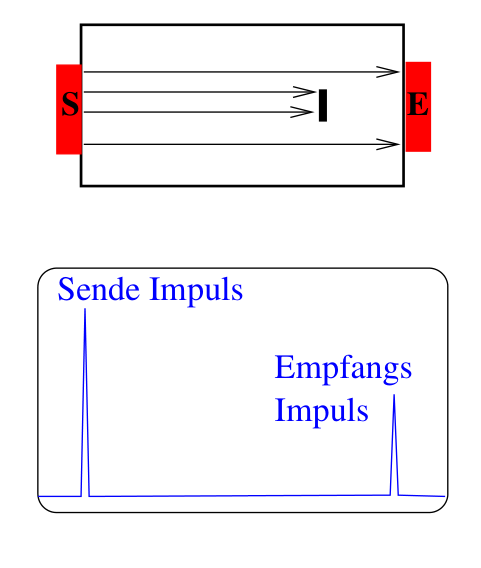
\includegraphics[height=8cm]{Pics/Durchschall.png}
      \caption{Durchschall-Verfahren}
      \label{fig:Durchschall}
  \end{subfigure}
  \begin{subfigure}{0.48\textwidth}
    \centering
      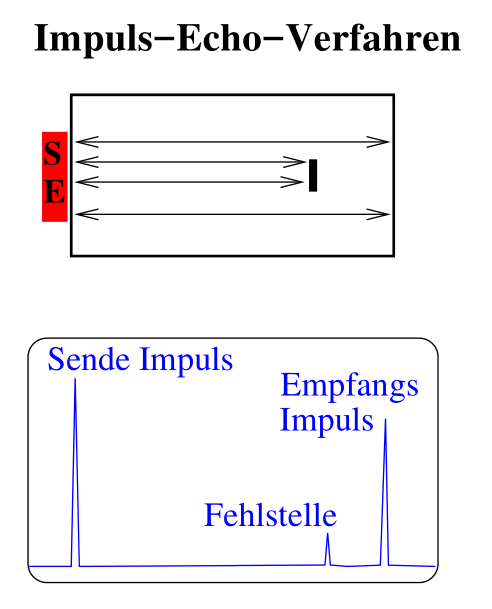
\includegraphics[height=8cm]{Pics/Impuls_Echo.png}
      \caption{Impuls-Echo-Verfahren}
      \label{fig:Impuls_Echo}
    \end{subfigure}
\caption{Die beiden Messmethoden für US1. \cite{anleitung01}}
\label{fig:Messmethoden}
\end{figure}

Für beide Verfahren gibt es verschiedenen Darstellungsmöglichkeiten, den A-Scan,
den B-Scan und den TM-Scan. Bei dem A-Scan (Amplitude-Scan) wird auf einem
Bildschirm die Amplitude der registrierten Welle dargestellt. Bei dem B-Scan
(Brightness-Scan) wird hingegen die aufgenommene Amplitude in eine Helligkeitsstufe
umgewandelt, sodass durch viele punktuelle Messungen ein 2-dimensionales Bild
eines Mediums aufgenommen werden kann. Beim TM-Scan (Time-Scan) wird eine hohe
Impulswiederholungsfrequenz verwendet, sodass zum Beispiel Bewegungen des Gewebes
durch unterschiedliche Impulsechos registriert werden und zeitlich dargestellt
werden können. Diese Scan-Methode wird häufig in der Medizin kombiniert mit dem
B-Scan angewandt.

\section{Versuchsaufbau und Versuchsdurchführung}

\subsection{Versuchsaufbau}

Die grundlegenden Bestandteile des Aufbaus sind ein Echoskop, zwei Ultraschallsonden,
ein PC zur Auswertung der Daten, sowie verschiedene Acrylplatten und -Zylinder.
Das Echoskop kann ausschließlich im Impuls-Betrieb genutzt werden. Zwischen den
beiden Scan-Einstellungen (siehe Abschnitt 1.1) kann mit einem Kipp-Schalter
gewechselt werden, indem der Schalter auf \textbf{REFLEC.} oder \textbf{TRANS.}
umgelegt wird. Für den Versuch werden zwei Ultraschallsonden mit 2 MHz verwendet,
deren Empfangsleistung zwischen 0 und 35 dB liegen.

Bei der verwendeten Messsoftware handelt es sich um das Programm Echo-View, mit
dem sowohl A-Scan, FFT Spektrum, Cepstrum und das Verstärkung TGC betrachtet
werden kann. Mithilfe der beiden Cursor können Differenzen zwischen zwei Positionen
auf der X-Achse bestimmt werden. Zudem geben diese beiden Cursor das Intervall
an, welches für das Frequenzspektrum und das Cepstrum verwendet werden.
Bei dem A-Scan kann das Signal sowohl als Funktion der Zeit (in $\si{\micro\second}$)
als auch als Funktion der Eindringtiefe (in mm) betrachtet werden. Mithilfe der
Freeze- und Start-Taste kann die durchgehende Aktualisierung des A-Scan-Bildes
zudem angehalten und wieder gestartet werden.

Mit der Time Gain Control kann die Verstärkung über die Parameter Treshhold, Wide,
Slope und Start eingestellt weren. Die erstellte Grafik kann mit Export abgespeichert
werden.


\subsection{Versuchsdurchführung}

Für den Versuch werden im Vorhinein schon die Schallgeschwindigkeiten von verschiedenen
Medien recherchiert, unter anderem von Acryl. Als erstes wird die rausgesuchte
Schallgeschwindigkeit in das Programm eingegeben und mittels
Impuls-Echo-Verfahren die Tiefenmessung überprüft.
Dafür wird die mit einer Schieblehre bestimmte Länge eines Acrylzylinders
mit dem Wert aus der Tiefenmessung verglichen.

Anschließend wird mit dem Impuls-Echo-Verfahrens die Laufzeit von verschiedenen
Acrylzylindern bestimmt. Dafür wird ein Zylinder auf ein Papiertuch gestellt und
mit bidestilliertem Wasser an eine $\SI{2}{MHz}$ Sonde gekoppelt. Mittels eines
A-Scans und den Cursorn wird die zeitliche Distanz zwischen dem ausgesandten und
dem reflektierten Signal gemessen.
Des Weiteren werden die Amplituden der verschiedenen Peaks gemessen, um
daraus die Dämpfung zu bestimmen. Um die Messung nicht zu verfälschen, wird dafür
die Verstärkung bei dem Versuch komplett ausgeschaltet. Die Messung wird anschließend
für 7 weitere Zylinder wiederholt.

Im nächsten Teil des Experimentes wird die Durchlaufzeit noch einmal mit der
Durchschall-Methode gemessen. Dafür wird der Zylinder auf eine Schiene gelegt und
an beide Enden werden mit Hydrogel Ultraschallsonden gekoppelt. Auf dem
A-Scan wird dann wieder die Laufzeit abgelesen, indem erneut der zeitliche
Abstand zwischen den Peaks mit den Cursor ausgemessen wird.

Im weiteren Verlauf des Versuchs werden zwei Acrylscheiben verschiedener Dicke
auf ein Papiertuch gelegt und mit bidestilliertem Wasser gekoppelt. Anschließend
wird noch ein Zylinder auf beide Scheiben gestellt und eine Sonde angekoppelt.
Um die Mehrfachreflexion mittels des Impuls-Echo-Verfahren deutlich erkennen zu
können, wird die Verstärkung
solange erhöht, bis mindestens drei Reflexionen erkennbar sind. Mittels der Cursor
wird wieder der zeitliche Abstand zwischen den Peaks gemessen. Zusätzlich werden
das Spektrum und das Cepstrum erstellt und abgespeichert.

Im letzten Teil des Experimentes wird noch einmal das Auge (Abb. \ref{fig:Auge}) untersucht. Dafür wird
erneut das Impuls-Echo-Verfahren genutzt. Die $\SI{2}{MHz}$ Sonde wird mit dem
Hydrogel an das Auge gekoppelt und solange leicht verschoben, bis auf dem A-Scan-Bild
mehrere Peaks erkennbar sind. Anschließend werden wieder die zeitlichen Abstände
mittels der Cursor vermessen und notiert, sowie ein A-Scan-Bild exportiert.

\begin{figure}
  \centering
  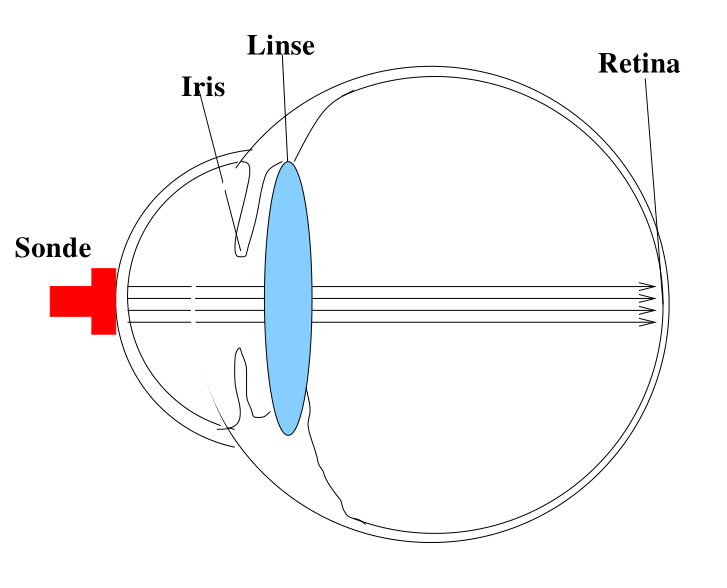
\includegraphics[width=0.7\textwidth]{Pics/Auge.png}
  \caption{Schematischer Aufbau des zu untersuchenden Augenmodells \cite{anleitung01}.}
  \label{fig:Auge}
\end{figure}
